\input{../templates/course_definitions}
\input{../templates/course_information}
\usepackage{csquotes}
\usepackage{tikz}
\usepackage{tikz-qtree}

\title{Java}
\subtitle{Scopes, Reference \& JavaDoc}
\date{\today}

\begin{document}

\begin{frame}
\titlepage
\end{frame}

\begin{frame}{Überblick}
    \setbeamertemplate{section in toc}[sections numbered]
    \tableofcontents
\end{frame}

\section{Scopes}

\begin{frame}[fragile]{Scopes}
    \center
    \large{Variablen sind nur innerhalb des Kontexts(d.h. innerhalb der \texttt{\{\}}) verfügbar, in denen sie deklariert wurden. \\
    \pause
    Das ist alles.}
    \pause
    \begin{columns}[T]
        \begin{column}{.5\textwidth}
            Richtig:
            \begin{lstlisting}[gobble=16]
                public class Scope {
                    int a = 5;
                    if(a <= 6) {
                        float f = (float)a;
                        System.out.println(f/1.25f);
                    }
                    System.out.println(a*10);
                }
            \end{lstlisting}
        \end{column}
        \begin{column}{.5\textwidth}
            Falsch:
            \begin{lstlisting}[gobble=16]
                public class Scope {
                    int a = 5;
                    if(a == 6) {
                        float f = (float)a;
                    }
                    System.out.println(f/1.25f);
                    //f is only available inside the if block
                    System.out.println(a*10);
                }
            \end{lstlisting}
        \end{column}
    \end{columns}
\end{frame}

\section{Die Reference}
\subsection{Intro}

\begin{frame}{Die Java-Reference}
    Die Java-Standardbibliothek ist in der sogenannten \textit{Reference} dokumentiert. Jede Java-Version hat ihre eigene Version der Reference;
    die momentan aktuellste Version(Java 10) ist unter \small\url{https://docs.oracle.com/javase/10/docs/api/overview-summary.html} \normalsize zu finden.\\
    \pause
    Die Reference ist hierarchisch gegliedert: \\
    \smallskip \small
    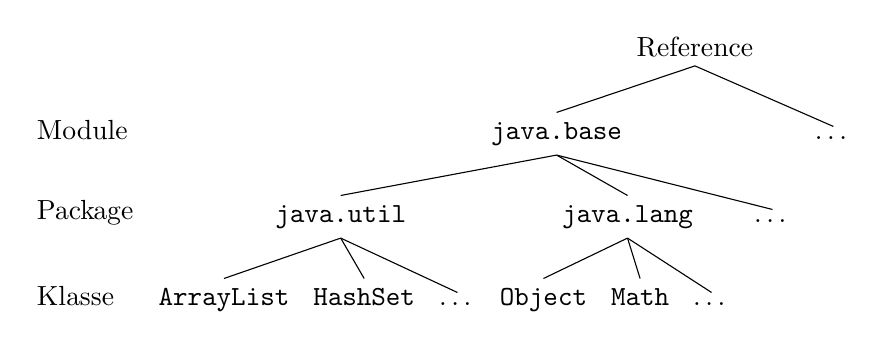
\begin{tikzpicture}
        \Tree   [.Reference 
                    [.\node (level0) {\texttt{java.base}}; 
                        [.\node (level1) {\texttt{java.util}}; 
                            \node (level2) {\texttt{ArrayList}}; {\texttt{HashSet}} {\dots}
                        ] 
                        [.{\texttt{java.lang}}
                            {\texttt{Object}} {\texttt{Math}} {\dots}
                        ]
                        {\dots}
                    ]
                    {\dots}
                ]
            \foreach \Value/\Text in {0/{Module},1/{Package},2/{Klasse}}
            {  
              \node[anchor=west] 
                at ([xshift=-2.5cm,yshift=0.05cm]{level2}|-{level\Value}) 
                {\Text};
            }
    \end{tikzpicture}
\end{frame}

\begin{frame}{Struktur einer Reference-Seite}
    Die Seite einer einzelnen Klasse(oder eines Interfaces) in der Reference ist folgendermaßen strukturiert:
    \begin{enumerate}[<+->]
        \item Eine kurze Zusammenfassung der Klasse, bestehend aus: 
            \begin{itemize}
                \item Der \enquote{Vererbungshierarchie} der Klasse
                \item Gegebenenfalls generische Typvariablen der Klasse
                \item Alle implementierten Interfaces \& alle bekannten erbenden Klassen
                \item Alle Super- und Subinterfaces(nur für Interfaces)
                \item Alle bekannten implementierenden Klassen(nur für Interfaces)
                \item 
            \end{itemize}
    \end{enumerate}
\end{frame}

\end{document}
